\documentclass[a4paper]{report}
\pagestyle{headings}
\usepackage{hyperref}
\usepackage{listings}
\usepackage{graphicx}
\lstset{language=bash}
\lstset{numbers=right}
\lstset{breaklines}
\title{Lab Report for Object-oriented Programming course \newline
 Lab 3: Linkage}
\author{Wang, Chen \\ 16307110064 \\ School of Software\\ Fudan University}
\date{\today}
\bibliographystyle{plain}
\begin{document}
\maketitle

\tableofcontents

\chapter{Background Knowledge \& Concepts Required for This Lab}
\section{C/C++ Compiling Process}

\subsection{Overall process of compiling}
Compiling a source code file in C++ is a four-step process.\footnote{Referenced from the website of \url{http://faculty.cs.niu.edu/mcmahon/CS241/Notes/compile.html} on April 18, 2019}
 For example, if you have a C++ source code file named \emph{prog1.cpp} and you execute the compile command
 \begin{lstlisting}[language=bash]
g++ -Wall -std=c++11 -o prog1 prog1.cpp
\end{lstlisting}
the compilation process looks like this:
\begin{enumerate}
\item
The C++ preprocessor copies the contents of the included header files into the source code file, generates macro code, and replaces symbolic constants defined using \emph{\#define} with their values.
\item
The expanded source code file produced by the C++ preprocessor is compiled into the assembly language for the platform.
\item
The assembler code generated by the compiler is assembled into the object code for the platform.
\item
The object code file generated by the assembler is linked together with the object code files for any library functions used to produce an executable file.
\end{enumerate}
By using appropriate compiler options, we can stop this process at any stage.
\begin{enumerate}
\item
To stop the process after the preprocessor step, you can use the \emph{-E} option:
\begin{lstlisting}[language=bash]
g++ -Wall -std=c++11 -E prog1.cpp
\end{lstlisting}

The expanded source code file will be printed on standard output (the screen by default); you can redirect the output to a file if you wish. Note that the expanded source code file is often incredibly large - a 20 line source code file can easily produce an expanded file of 20,000 lines or more, depending on which header files were included.
\item
To stop the process after the compile step, you can use the \emph{-S} option:

\begin{lstlisting}[language=bash]
g++ -Wall -std=c++11 -S prog1.cpp
\end{lstlisting}

By default, the assembler code for a source file named \emph{filename.cpp} will be placed in a file named \emph{filename.s}.
\item
To stop the process after the assembly step, you can use the \emph{-c} option:
\begin{lstlisting}[language=bash]
g++ -Wall -std=c++11 -c prog1.cpp
\end{lstlisting}

By default, the assembler code for a source file named \emph{filename.cpp} will be placed in a file named \emph{filename.o}.
The entire process for compiling is shown in the figure \ref{1}
\begin{figure}
  \centering
  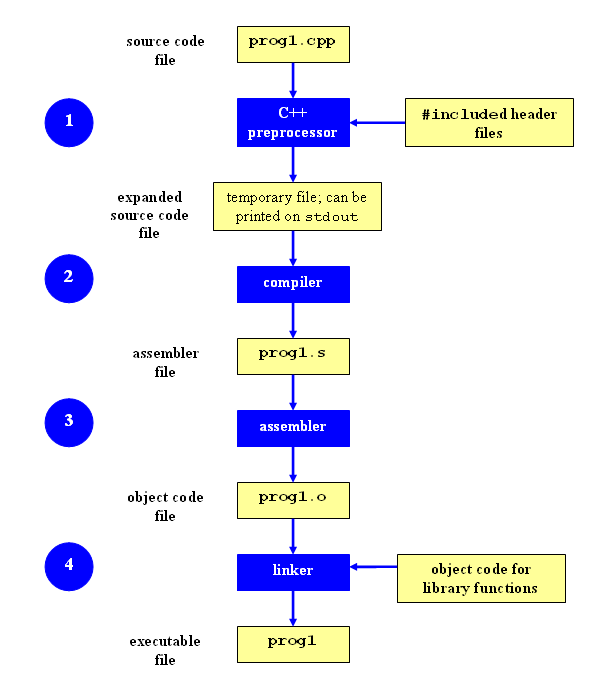
\includegraphics[width=12cm]{compile.png}
  \caption{Overall compiling process}\label{1}
\end{figure}
\end{enumerate}

\subsection{Preprocessing}
To program in C and C++, you need to understand the steps and tools in the compilation process. Some languages (C and C++, in particular) start compilation by running a \emph{preprocessor} on the source code. The preprocessor is a simple program that replaces patterns in the source code with other patterns the programmer has defined (using \emph{preprocessor directives}). Preprocessor directives are used to save typing and to increase the readability of the code. However, from the author of the book TIC, the design of C++ is meant to discourage much of the use of the preprocessor, since it can cause subtle bugs. The pre-processed code is often written to an intermediate file. 
\subsection{Parsing}
Compilers usually do their work in two passes. The first pass \emph{parses} the pre-processed code. The compiler breaks the source code into small units and organizes it into a structure called a \emph{tree}. In the expression “\textbf{A + B}” the elements ‘\textbf{A}’, ‘\textbf{+},’ and ‘\textbf{B}’ are leaves on the parse tree. 
\subsection{Global optimization}
A \emph{global optimizer} is sometimes used between the first and second passes to produce smaller, faster code. 
\subsection{Code generation}
In the second pass, the \emph{code generator} walks through the parse tree and generates either assembly language code or machine code for the nodes of the tree. If the code generator creates assembly code, the assembler must then be run. The end result in both cases is an object module (a file that typically has an extension of \textbf{.o} or \textbf{.obj}).
\subsection{Peehole optimization}
 A \emph{peephole optimizer} is sometimes used in the second pass to look for pieces of code containing redundant assembly-language statements. 
\subsection{Linking}
The use of the word “object” to describe chunks of machine code is an unfortunate artifact. The word came into use before objectoriented programming was in general use. “Object” is used in the same sense as “goal” when discussing compilation, while in objectoriented programming it means “a thing with boundaries.” 
\par
The \emph{linker} combines a list of object modules into an executable program that can be loaded and run by the operating system. When a function in one object module makes a reference to a function or variable in another object module, the linker resolves these references; it makes sure that all the external functions and data you claimed existed during compilation do exist. The linker also adds a special object module to perform start-up activities. 
\par
The linker can search through special files called \emph{libraries} in order to resolve all its references. A library contains a collection of object modules in a single file. A library is created and maintained by a program called a \emph{librarian}. 
\section{Preprocessing}
\subsection{The need of preprocessing}
In computer science, a \textbf{preprocessor} is a program that processes its input data to produce output that is used as input to another program. The output is said to be a \textbf{preprocessed} form of the input data, which is often used by some subsequent programs like compilers. The amount and kind of processing done depends on the nature of the preprocessor; some preprocessors are only capable of performing relatively simple textual substitutions and macro expansions, while others have the power of full-fledged programming languages. 
A common example from computer programming is the processing performed on source code before the next step of compilation. In some computer languages (e.g., C and PL/I) there is a phase of translation known as \emph{preprocessing}. It can also include macro processing, file inclusion and language extensions. 

\subsection{Different preprocessing algorithms}
Preprocessors can be divided into different types: lexical preprocessors, syntactic preprocessors and general purpose preprocessors. Each type will be further discussed in the following subsections.
\subsection{Lexical preprocessors}
Lexical preprocessors are the lowest-level of preprocessors as they only require lexical analysis, that is, they operate on the source text, prior to any parsing, by performing simple substitution of tokenized character sequences for other tokenized character sequences, according to user-defined rules. They typically perform macro substitution, textual inclusion of other files, and conditional compilation or inclusion. 
\par
The most common example of this is the C preprocessor, which takes lines beginning with `\#' as directives. Because it knows nothing about the underlying language, its use has been criticized and many of its features built directly into other languages. For example, macros replaced with aggressive inlining and templates, includes with compile-time imports (this requires the preservation of type information in the object code, making this feature impossible to retrofit into a language); conditional compilation is effectively accomplished with if-then-else and dead code elimination in some languages. However, a key point to remember is that all preprocessor directives should start on a new line. 
\par
Other lexical preprocessors include the general-purpose m4, most commonly used in cross-platform build systems such as autoconf, and GEMA, an open source macro processor which operates on patterns of context. 

\subsection{Syntactic preprocessors}
Syntactic preprocessors were introduced with the Lisp family of languages. Their role is to transform syntax trees according to a number of user-defined rules. For some programming languages, the rules are written in the same language as the program (compile-time reflection). This is the case with Lisp and OCaml. Some other languages rely on a fully external language to define the transformations, such as the XSLT preprocessor for XML, or its statically typed counterpart CDuce.
\par
Syntactic preprocessors are typically used to customize the syntax of a language, extend a language by adding new primitives, or embed a domain-specific programming language (DSL) inside a general purpose language. 

\subsection{General purpose preprocessor}
Most preprocessors are specific to a particular data processing task (e.g., compiling the C language). A preprocessor may be promoted as being \emph{general purpose}, meaning that it is not aimed at a specific usage or programming language, and is intended to be used for a wide variety of text processing tasks. 
\par
M4 is probably the most well known example of such a general purpose preprocessor, although the C preprocessor is sometimes used in a non-C specific role.
\subsection{Preprocessing algorithm utilized by the current g++}
The \textbf{C preprocessor} or \textbf{cpp} is the macro preprocessor for the C and C++ computer programming languages. The preprocessor provides the ability for the inclusion of header files, macro expansions, conditional compilation, and line control. 
\par
In many C implementations, it is a separate program invoked by the compiler as the first part of translation. 
\par
The language of preprocessor directives is only weakly related to the grammar of C, and so is sometimes used to process other kinds of text files. 
\par
Preprocessing is defined by the first four (of eight) \emph{phases of translation} specified in the C Standard. 
\begin{enumerate}
\item
Trigraph replacement: The preprocessor replaces trigraph sequences with the characters they represent.
\item
Line splicing: Physical source lines that are continued with escaped newline sequences are \emph{spliced} to form logical lines.
\item
Tokenization: The preprocessor breaks the result into \emph{preprocessing tokens} and whitespace. It replaces comments with whitespace.
\item
Macro expansion and directive handling: Preprocessing directive lines, including file inclusion and conditional compilation, are executed. The preprocessor simultaneously expands macros and, in the 1999 version of the C standard, handles \textbf{\_Pragma} operators.
\end{enumerate}
\par
However, in this lab we are not required to accomplish all the steps of the C preprocessor program and the test case only cover a small part of the required tasks of a C/C++ preprocessor. The details of this lab are shown in the consequent chapters.
\chapter{Tasks of This Lab}
\section{Understanding Internal and External Linkage}
%





The experiment requires a source code preprocessor to implement precompilation of macro directives in the code file. The preprocessor will process the macro definitions in the code before the code is compiled. Common instructions are: \#include, \#define, \#undef, \#ifdef, \#ifndef, \#if, \#endif and so on.
\par
You can use \emph{g++ -E test1.cpp > output.cpp} to see the code after \emph{test1.cpp} is precompiled in \emph{output.cpp}. In this lab, you need to implement a precompiled processor (without needing to deal with the C++ standard library) to handle instruction precompilation in simple scenarios.
\section{Understanding Name Space}
\begin{enumerate}
\item
Implementation: In the lab we need to write our code in \emph{lab2.cpp}. \emph{lab2.cpp} provides an entry function, we need to implement our code at this entry location.
\item
Test: There are two cpp test files in the test folder. \emph{Test1.cpp} is very simple and can help us debug at an early stage. \emph{Test2.cpp} is relatively complex and requires us to carefully identify the various macro processing scenarios.
\item
Run: First we need to compile \emph{lab2.cpp} (compiled with c++11 standard), and run the compiled file. After running, two \emph{test.out.cpp} files are generated in the test folder. Then run the \emph{run\_tests.sh} file in the test folder and make sure we are in the test directory before running this file.
\end{enumerate}
\section{Compare with Typescript Name Space}
The test cases in this lab are designed to check the following directives.
\begin{itemize}
\item \#include – 10\% (do not need to deal with \textbf{\#include "iostream"})
\item \#define (check1 to check5)– 10\%
\item \#undef – 10\%
\item \#ifdef – 10\%
\item \#else – 10\%
\item \#ifndef – 10\%
\item \#if – 10\%
\item \#define function(PART 2) – 10\%
\item \#define function(PART 3) – 10\% (for 5\% and \#\# processing, \_\# and \#\# can be processed as long as they can pass the test file)
\item \textbf{No memory leaks - 10\%}
\end{itemize}

\chapter{Structure and  the OO Ideas Adopted}
\section{Objected-oriented ideas adopted in the implementation}
\subsection{Encapsulation}
Encapsulation \emph{is one of the fundamentals} of OOP (object-oriented programming). It refers to the bundling of data with the methods that operate on that data. Encapsulation is \emph{used to hide the values or state of a structured data object inside a class}, preventing unauthorized parties' direct access to them. Publicly accessible methods are generally provided in the class (so-called \emph{getters} and \emph{setters}) to access the values, and other client classes call these methods to retrieve and modify the values within the object. 
This mechanism is not unique to object-oriented programming. Implementations of abstract data types, e.g. modules, offer a similar form of encapsulation. This similarity stems from the fact that both notions rely on the same mathematical fundamental of an existential type.
\subsection{Encapsulated data structure in this lab}
The encapsulation result of the class is shown as Figure \ref{2}. From the structure, we can see that only the necessary constructor, destructor and the entry method \emph{pre\_process} are \textbf{public}. All the class fields and the other helper methods are \textbf{private}.
\begin{figure}
  \centering
  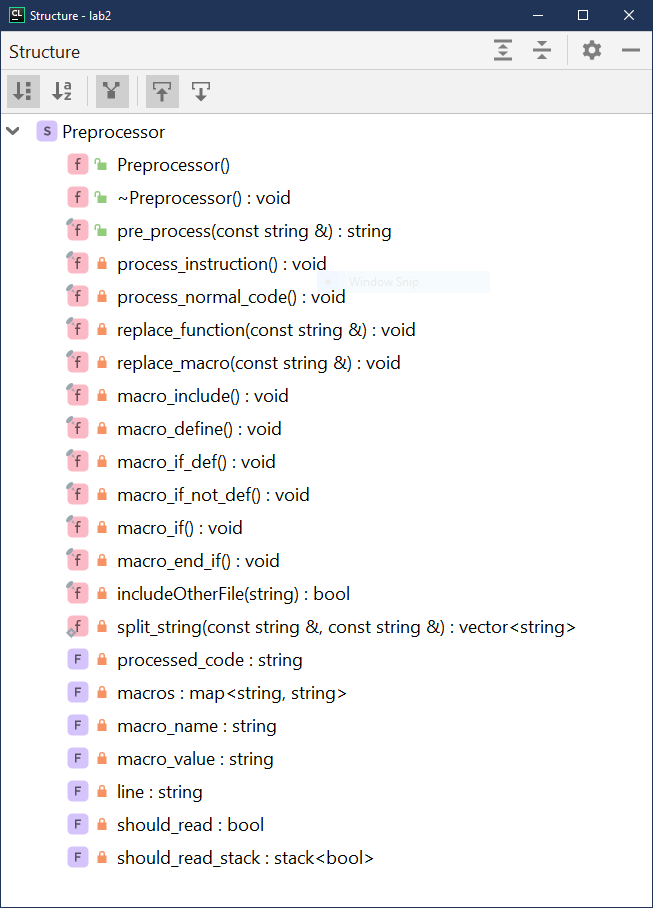
\includegraphics[scale=0.6]{structure.png}
  \caption{Encapsulated class structure}\label{2}
\end{figure}
\chapter{Running Result of My Implementation}
The following screenshots are the tests that are identical to the steps in the requirement documentation and proves that my version of implementation functions identical to the standard version.
\section{Test result of the testcases}
The results are shown as Figure \ref{3}. The \emph{out} processed files are in the \emph{test} sub folder.
\begin{figure}
  \centering
  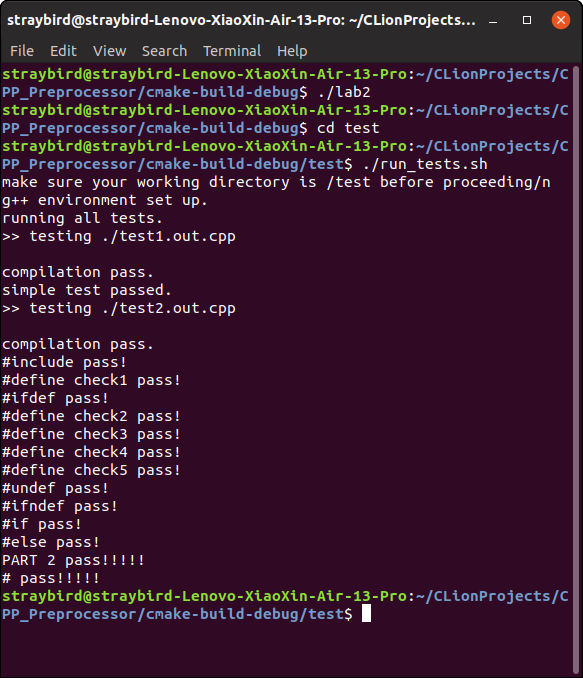
\includegraphics[width=12cm]{shell.png}
  \caption{Testcase Result}\label{3}
\end{figure}

\chapter{Memory Leak}
\section{Potential Memory Leak}
In computer science, a \textbf{memory leak} is a type of resource leak that occurs when a computer program incorrectly manages memory allocations in such a way that memory which is no longer needed is not released. A memory leak may also happen when an object is stored in memory but cannot be accessed by the running code. A memory leak has symptoms similar to a number of other problems and generally can only be diagnosed by a programmer with access to the programs' source code. 
\par
A space leak occurs when a computer program uses more memory than necessary. In contrast to memory leaks, where the leaked memory is never released, the memory consumed by a space leak is released, but later than expected.
\par
Because they can exhaust available system memory as an application runs, memory leaks are often the cause of or a contributing factor to software aging.
\section{Prove of Free from Memory Leak in my Implementation}
\subsection{Tools adopted for analysis: Valgrind}
Valgrind is an instrumentation framework for building dynamic analysis tools. There are Valgrind tools that can automatically detect many memory management and threading bugs, and profile your programs in detail. You can also use Valgrind to build new tools. 
\par
The Valgrind distribution currently includes six production-quality tools\footnote{Referenced from the website of Valgrind on April 18, 2019: \url{http://valgrind.org}}: a memory error detector, two thread error detectors, a cache and branch-prediction profiler, a call-graph generating cache and branch-prediction profiler, and a heap profiler. It also includes three experimental tools: a stack/global array overrun detector, a second heap profiler that examines how heap blocks are used, and a SimPoint basic block vector generator. It runs on the following platforms: X86/Linux, AMD64/Linux, ARM/Linux, ARM64/Linux, PPC32/Linux, PPC64/Linux, PPC64LE/Linux, S390X/Linux, MIPS32/Linux, MIPS64/Linux, X86/Solaris, AMD64/Solaris, ARM/Android (2.3.x and later), ARM64/Android, X86/Android (4.0 and later), MIPS32/Android, X86/Darwin and AMD64/Darwin (Mac OS X 10.12).
\par
Valgrind is Open Source / Free Software, and is freely available under the GNU General Public License, version 2.
\par
In this lab, I only used the memory check tool to analyze whether there are any potential memory leaks in my application.
\subsection{Result of the memory check}
From Figure \ref{4} above, we can see that there is no memory leak found in my application.
\begin{figure}
  \centering
  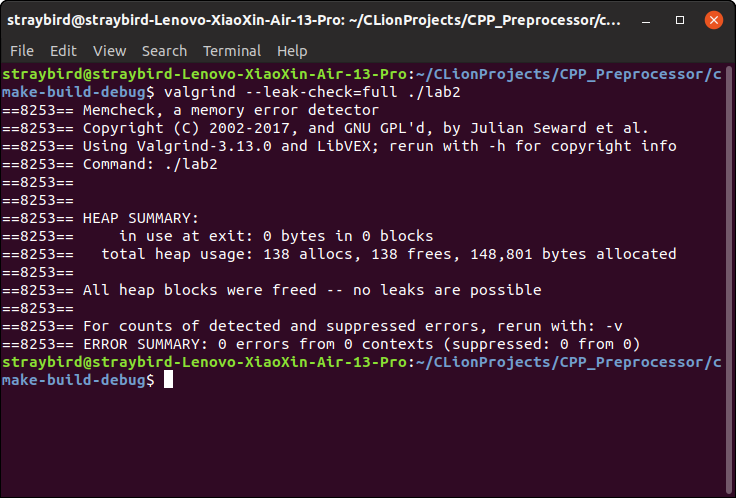
\includegraphics[width=12cm]{mem.png}
  \caption{Memory Leak Check Result: No memory leak found}\label{4}
\end{figure}
\begin{thebibliography}{A}

\bibitem{1}
Wikipedia contributors. (2019, February 3). Encapsulation (computer programming). In \emph{Wikipedia, The Free Encyclopedia}. Retrieved 10:19, March 23, 2019, from \url{https://en.wikipedia.org/w/index.php?title=Encapsulation_(computer_programming)&oldid=881507936}

\bibitem{2}
Wikipedia contributors. (2019, March 17). Reversi. In \emph{Wikipedia, The Free Encyclopedia}. Retrieved 10:20, March 23, 2019, from \url{https://en.wikipedia.org/w/index.php?title=Reversi&oldid=888167585}

\bibitem{3}
Wikipedia contributors. (2019, March 15). Polymorphism (computer science). In \emph{Wikipedia, The Free Encyclopedia}. Retrieved 10:21, March 23, 2019, from \url{https://en.wikipedia.org/w/index.php?title=Polymorphism_(computer_science)&oldid=887878749}

\bibitem{4}
Wikipedia contributors. (2019, February 27). Object-oriented programming. In \emph{Wikipedia, The Free Encyclopedia}. Retrieved 10:22, March 23, 2019, from \url{https://en.wikipedia.org/w/index.php?title=Object-oriented_programming&oldid=885274966}

\bibitem{5}
Wikipedia contributors. (2019, February 21). Inheritance (object-oriented programming). In \emph{Wikipedia, The Free Encyclopedia}. Retrieved 10:22, March 23, 2019, from \url{https://en.wikipedia.org/w/index.php?title=Inheritance_(object-oriented_programming)&oldid=884436146}

\end{thebibliography}
\end{document} 